\section{Delta-function}

In complex analysis, we have the identity
\[
\int_{-\infty}^{\infty} e^{ itx } \, dx =2\pi\delta_0(t)
\]
In logic, this is not a consequence from the Fourier analysis but from the contour integration.

\begin{figure}[H]
\centering
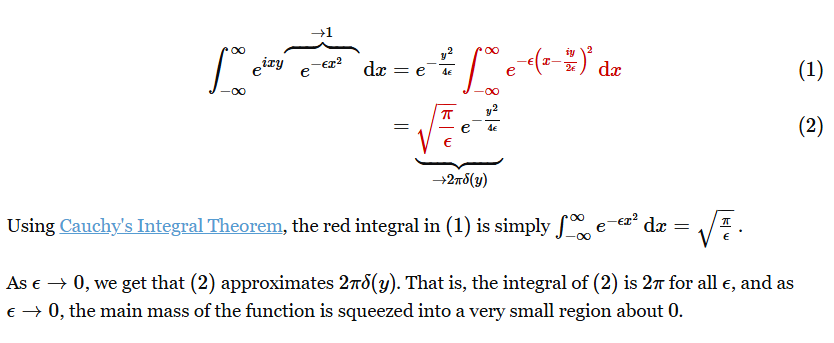
\includegraphics[width=\textwidth]{1-delta-function-20250313.png}
% \caption{}
\label{}
\end{figure}

It suffices to show that
\[
\int_{-\infty}^{\infty} e^{ -(x+ik)^{2} } \, dx=\int_{-\infty }^{\infty} e^{ -x^{2} } \, dx=\sqrt{ \pi }
\]
Consider the toy contour:

\begin{figure}[H]
\centering
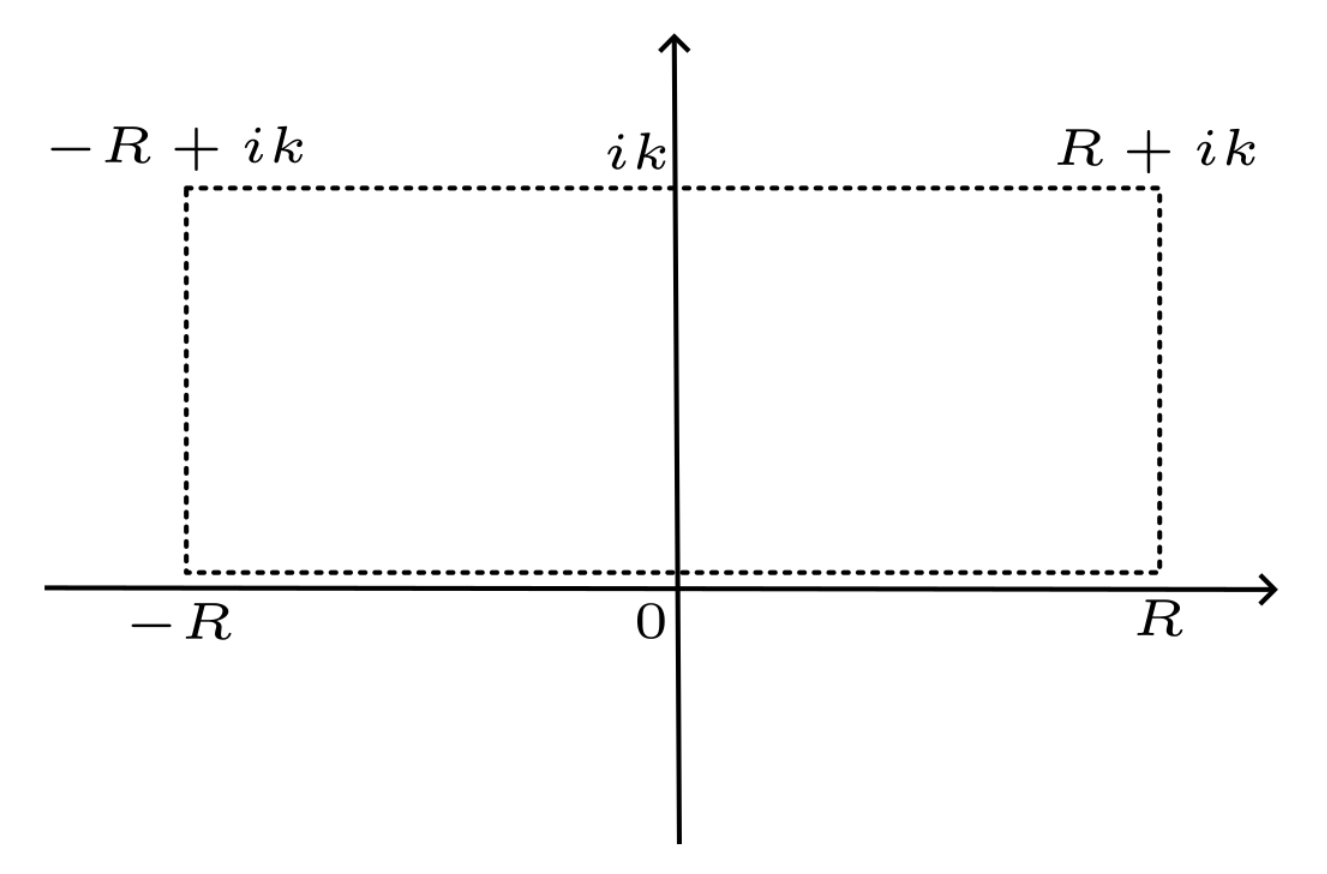
\includegraphics[width=\textwidth]{2-delta-function-20250313.png}
% \caption{}
\label{}
\end{figure}
\[
\int_{-R}^{R}+\int_{R}^{R+ik}-\int_{-R+ik}^{R+ik}-\int_{-R}^{-R+ik} e^{ -z^{2} } \, dz=0 
\]
Since
\[
\left\lvert  \int_{R}^{R+ik} e^{ -z^{2} } \, dz   \right\rvert \leq \int_{R}^{R+ik} \lvert e^{ -z^{2} } \rvert  \, dz =\int_{0}^{k} \lvert e^{ -(R+ix)^{2} } \rvert  \, dx \leq ke^{ -R^{2} }\to0\qquad \text{as }R\to \infty
\]
\[
\lim_{ R \to \infty } \int_{-R}^{-R+ik} e^{ -z^{2} } \, dz =0
\]
We know that
\[
\lim_{ R \to \infty } \int_{-R}^{R} e^{ -x^{2} } \, dx=\lim_{ R \to \infty } \int_{-R+ik}^{R+ik} e^{ -z^{2} } \, dz =\lim_{ R \to \infty } \int_{-R}^{R} e^{ -(x+ik)^{2} } \, dx
\]
Therefore
\[
\int_{-\infty}^{\infty} e^{ -(x+ik)^{2} } \, dx =\int_{-\infty}^{\infty} e^{ -x^{2} } \, dx =\sqrt{ \pi }
\]